% 95-38(95쪽) — 지점 $\pt{O}$ 에서 $120^\circ$ 를 이루며 갈라져 나가는 두 로봇 $\pt{A}$, $\pt{B}$ 의 진로(원문 「오른쪽 그림」). 스캔 화질이 낮아 TikZ 로 다시 그림.
% 라벨은 원문 것만: $\pt{O}$·$\pt{A}$·$\pt{B}$·$120^\circ$ 와 진행 방향 화살표. 원문의 로봇 삽화는 수학 내용이 아니라 옮기지 않았다.
% 5초 후의 거리(답)가 읽히지 않게 선분 길이·눈금은 적지 않는다.
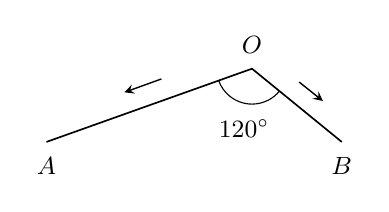
\begin{tikzpicture}[line width=0.6pt, >=stealth]
  \draw (-2.61,-0.93) -- (0,0) -- (1.14,-0.93);
  \draw[line width=0.4pt] (0.349,-0.284) arc (-39.2:-160.4:0.45);
  \draw[->, line width=0.5pt] (-1.15,-0.13) -- (-1.62,-0.30);
  \draw[->, line width=0.5pt] (0.60,-0.17) -- (0.90,-0.41);
  \node[font=\small] at (-0.10,-0.76) {$120^\circ$};
  \node[anchor=south, font=\small] at (0,0.06) {$\pt{O}$};
  \node[anchor=north, font=\small] at (-2.61,-1.00) {$\pt{A}$};
  \node[anchor=north, font=\small] at (1.14,-1.00) {$\pt{B}$};
\end{tikzpicture}
